\documentclass{beamer}
\usepackage[utf8]{inputenc}

\usetheme{Madrid}
\usecolortheme{default}
\usepackage{amsmath,amssymb,amsfonts,amsthm}
\usepackage{txfonts}
\usepackage{tkz-euclide}
\usepackage{listings}
\usepackage{adjustbox}
\usepackage{array}
\usepackage{tabularx}
\usepackage{gvv}
\usepackage{lmodern}
\usepackage{circuitikz}
\usepackage{tikz}
\usepackage{graphicx}

\setbeamertemplate{page number in head/foot}[totalframenumber]

\usepackage{tcolorbox}
\tcbuselibrary{minted,breakable,xparse,skins}



\definecolor{bg}{gray}{0.95}
\DeclareTCBListing{mintedbox}{O{}m!O{}}{%
  breakable=true,
  listing engine=minted,
  listing only,
  minted language=#2,
  minted style=default,
  minted options={%
    linenos,
    gobble=0,
    breaklines=true,
    breakafter=,,
    fontsize=\small,
    numbersep=8pt,
    #1},
  boxsep=0pt,
  left skip=0pt,
  right skip=0pt,
  left=25pt,
  right=0pt,
  top=3pt,
  bottom=3pt,
  arc=5pt,
  leftrule=0pt,
  rightrule=0pt,
  bottomrule=2pt,
  toprule=2pt,
  colback=bg,
  colframe=orange!70,
  enhanced,
  overlay={%
    \begin{tcbclipinterior}
    \fill[orange!20!white] (frame.south west) rectangle ([xshift=20pt]frame.north west);
    \end{tcbclipinterior}},
  #3,
}
\lstset{
    language=C,
    basicstyle=\ttfamily\small,
    keywordstyle=\color{blue},
    stringstyle=\color{orange},
    commentstyle=\color{green!60!black},
    numbers=left,
    numberstyle=\tiny\color{gray},
    breaklines=true,
    showstringspaces=false,
}
%------------------------------------------------------------
%This block of code defines the information to appear in the
%Title page
\title %optional
{1.9.15}
\date{August 22,2025}
%\subtitle{A short story}

\author % (optional)
{Harsha-EE25BTECH11026}



\begin{document}


\frame{\titlepage}
\begin{frame}{Question}
If a, b, c are position vectors of the points A$\brak{2, 3, -4}$, B$\brak{3, -4, -5}$, and C$\brak{3, 2, -3}$ respectively, then $\|a + b + c\|$ is equal to
\end{frame}



\begin{frame}{Theoretical Solution}

Given the position vectors,
\begin{align}
    \vec{a}=\begin{myvec}{2\\3\\4}\end{myvec}\;
    \vec{b}=\begin{myvec}{3\\-4\\-5}\end{myvec}\;
    \vec{c}=\begin{myvec}{3\\2\\-3}\end{myvec}
\end{align}
To find the magnitude of $\|a+b+c\|$,we can add these three vectors to find their sum, say S, and find their magnitude.

\end{frame}

\begin{frame}{Theoretical Solution}
\begin{align}
    \vec{S}=\vec{a}+\vec{b}+\vec{c}
\end{align}
\begin{align}
    \vec{S}=\begin{myvec}{2\\3\\-4}\end{myvec}+\begin{myvec}{3\\-4\\-5}\end{myvec}+\begin{myvec}{3\\2\\-3}\end{myvec}
\end{align}
\begin{align}
    \therefore\vec{S}=\begin{myvec}{8\\1\\-12}\end{myvec}
\end{align}
\end{frame}

\begin{frame}{Theoretical Solution}
The magnitude of S is given by \\
\begin{align}
    \|S\|^2=\vec{S}^T\vec{S}
\end{align}

\begin{align}
      \therefore\|S\|^2=\begin{myvec}{8&&1&&-12}\end{myvec}\begin{myvec}{8\\1\\-12}
      \end{myvec}
\end{align}
\begin{align}
    \|S\|^2=\myvec{209}
\end{align}
\begin{align}
    \therefore\|S\|=\myvec{14.457} \;units
\end{align}
\end{frame}

\begin{frame}[fragile]
    \frametitle{C Code - Sum of vectors and Magnitude of vectors}

    \begin{lstlisting}
#include<stdio.h>
#include<math.h>

double find_magnitude(int *result)
{
	double mag;
	mag=sqrt(pow(result[0],2)+pow(result[1],2)+pow(result[2],2));
	return mag;

}

void sum_of_vectors(int *a, int *b, int *c, int *result)
{
    for(int i = 0; i < 3; i++)
    {
        result[i] = a[i] + b[i] + c[i];
    }
}
    \end{lstlisting}
\end{frame}

\begin{frame}[fragile]
    \frametitle{Python+C Code}
    \begin{lstlisting}
import ctypes
import numpy as np
import matplotlib as mp
mp.use("TkAgg")  # must come before pyplot
import matplotlib.pyplot as plt

# Load C library
lib = ctypes.CDLL('./libmagnitude_sum.so')

# C function signatures
lib.sum_of_vectors.argtypes = [
    ctypes.POINTER(ctypes.c_int), 
    ctypes.POINTER(ctypes.c_int), 
    ctypes.POINTER(ctypes.c_int), 
    ctypes.POINTER(ctypes.c_int)
]
lib.sum_of_vectors.restype = None




    \end{lstlisting}
\end{frame}

\begin{frame}[fragile]
    \frametitle{Python+C Code}
    \begin{lstlisting}
lib.find_magnitude.argtypes = [ctypes.POINTER(ctypes.c_int)]
lib.find_magnitude.restype = ctypes.c_double

# Define vectors
A = np.array([2, 3, -4], dtype=np.int32)
B = np.array([3, -4, -5], dtype=np.int32)
C = np.array([3, 2, -3], dtype=np.int32)
S = np.zeros(3, dtype=np.int32)

# Sum vectors via C
lib.sum_of_vectors(
    A.ctypes.data_as(ctypes.POINTER(ctypes.c_int)),
    B.ctypes.data_as(ctypes.POINTER(ctypes.c_int)),
    C.ctypes.data_as(ctypes.POINTER(ctypes.c_int)),
    S.ctypes.data_as(ctypes.POINTER(ctypes.c_int))
)
    \end{lstlisting}
\end{frame}

\begin{frame}[fragile]
    \frametitle{Python+C Code}
    \begin{lstlisting}
print("Sum of vectors:", S)

# Magnitude via C
magnitude = lib.find_magnitude(S.ctypes.data_as(ctypes.POINTER(ctypes.c_int)))
print("Magnitude of sum vector: {:.3f}".format(magnitude))
    \end{lstlisting}
\end{frame}

\begin{frame}[fragile]
    \frametitle{Python+C Code}
    \begin{lstlisting}
# 3D Plot
origin = np.array([0,0,0])
fig = plt.figure(figsize=(8,8))
ax = fig.add_subplot(111, projection='3d')

ax.quiver(*origin, *A, color='r', label='A')
ax.quiver(*origin, *B, color='g', label='B')
ax.quiver(*origin, *C, color='b', label='C')
ax.quiver(*origin, *S, color='k', linewidth=2, label='Sum (A+B+C)')

max_val = max(np.abs(S)) + 2
ax.set_xlim([0, max_val])
ax.set_ylim([0, max_val])
ax.set_zlim([min(0, np.min(S)) - 2, max_val])
    \end{lstlisting}
\end{frame}
\begin{frame}[fragile]
    \frametitle{Python+C Code}
    \begin{lstlisting}
ax.set_xlabel('X')
ax.set_ylabel('Y')
ax.set_zlabel('Z')
ax.set_title('3D Vectors and their Sum')
ax.legend()

plt.savefig("/home/user/Matrix/Matgeo_assignments/1.9.15/figs/Figure_1.png", dpi=300, bbox_inches='tight')
plt.show()

    \end{lstlisting}
\end{frame}

\begin{frame}[fragile]
    \frametitle{Python Code}
    \begin{lstlisting}
import numpy as np
import matplotlib as mp
mp.use("TkAgg")  # must come before pyplot
import matplotlib.pyplot as plt

# Define vectors
A = np.array([2, 3, -4], dtype=np.int32)
B = np.array([3, -4, -5], dtype=np.int32)
C = np.array([3, 2, -3], dtype=np.int32)

# Sum of vectors
S = A + B + C
print("Sum of vectors:", S)


    \end{lstlisting}
\end{frame}

\begin{frame}[fragile]
    \frametitle{Python Code}
    \begin{lstlisting}
# Magnitude of sum vector
magnitude = np.linalg.norm(S)
print("Magnitude of sum vector: {:.3f}".format(magnitude))

# 3D Plot
origin = np.array([0, 0, 0])
fig = plt.figure(figsize=(8, 8))
ax = fig.add_subplot(111, projection='3d')

ax.quiver(*origin, *A, color='r', label='A')
ax.quiver(*origin, *B, color='g', label='B')
ax.quiver(*origin, *C, color='b', label='C')
ax.quiver(*origin, *S, color='k', linewidth=2, label='Sum (A+B+C)')

    \end{lstlisting}
\end{frame}

\begin{frame}[fragile]
    \frametitle{Python Code}
    \begin{lstlisting}
# Axis limits
max_val = max(np.abs(S)) + 2
ax.set_xlim([0, max_val])
ax.set_ylim([0, max_val])
ax.set_zlim([min(0, np.min(S)) - 2, max_val])

# Labels and title
ax.set_xlabel('X')
ax.set_ylabel('Y')
ax.set_zlabel('Z')
ax.set_title('3D Vectors and their Sum')
ax.legend()

# Save and show
plt.savefig("/home/user/Matrix/Matgeo_assignments/1.9.15/figs/Figure_1.png",
            dpi=300, bbox_inches='tight')
plt.show()

    \end{lstlisting}
\end{frame}

\begin{frame}{Plot}
    \centering
    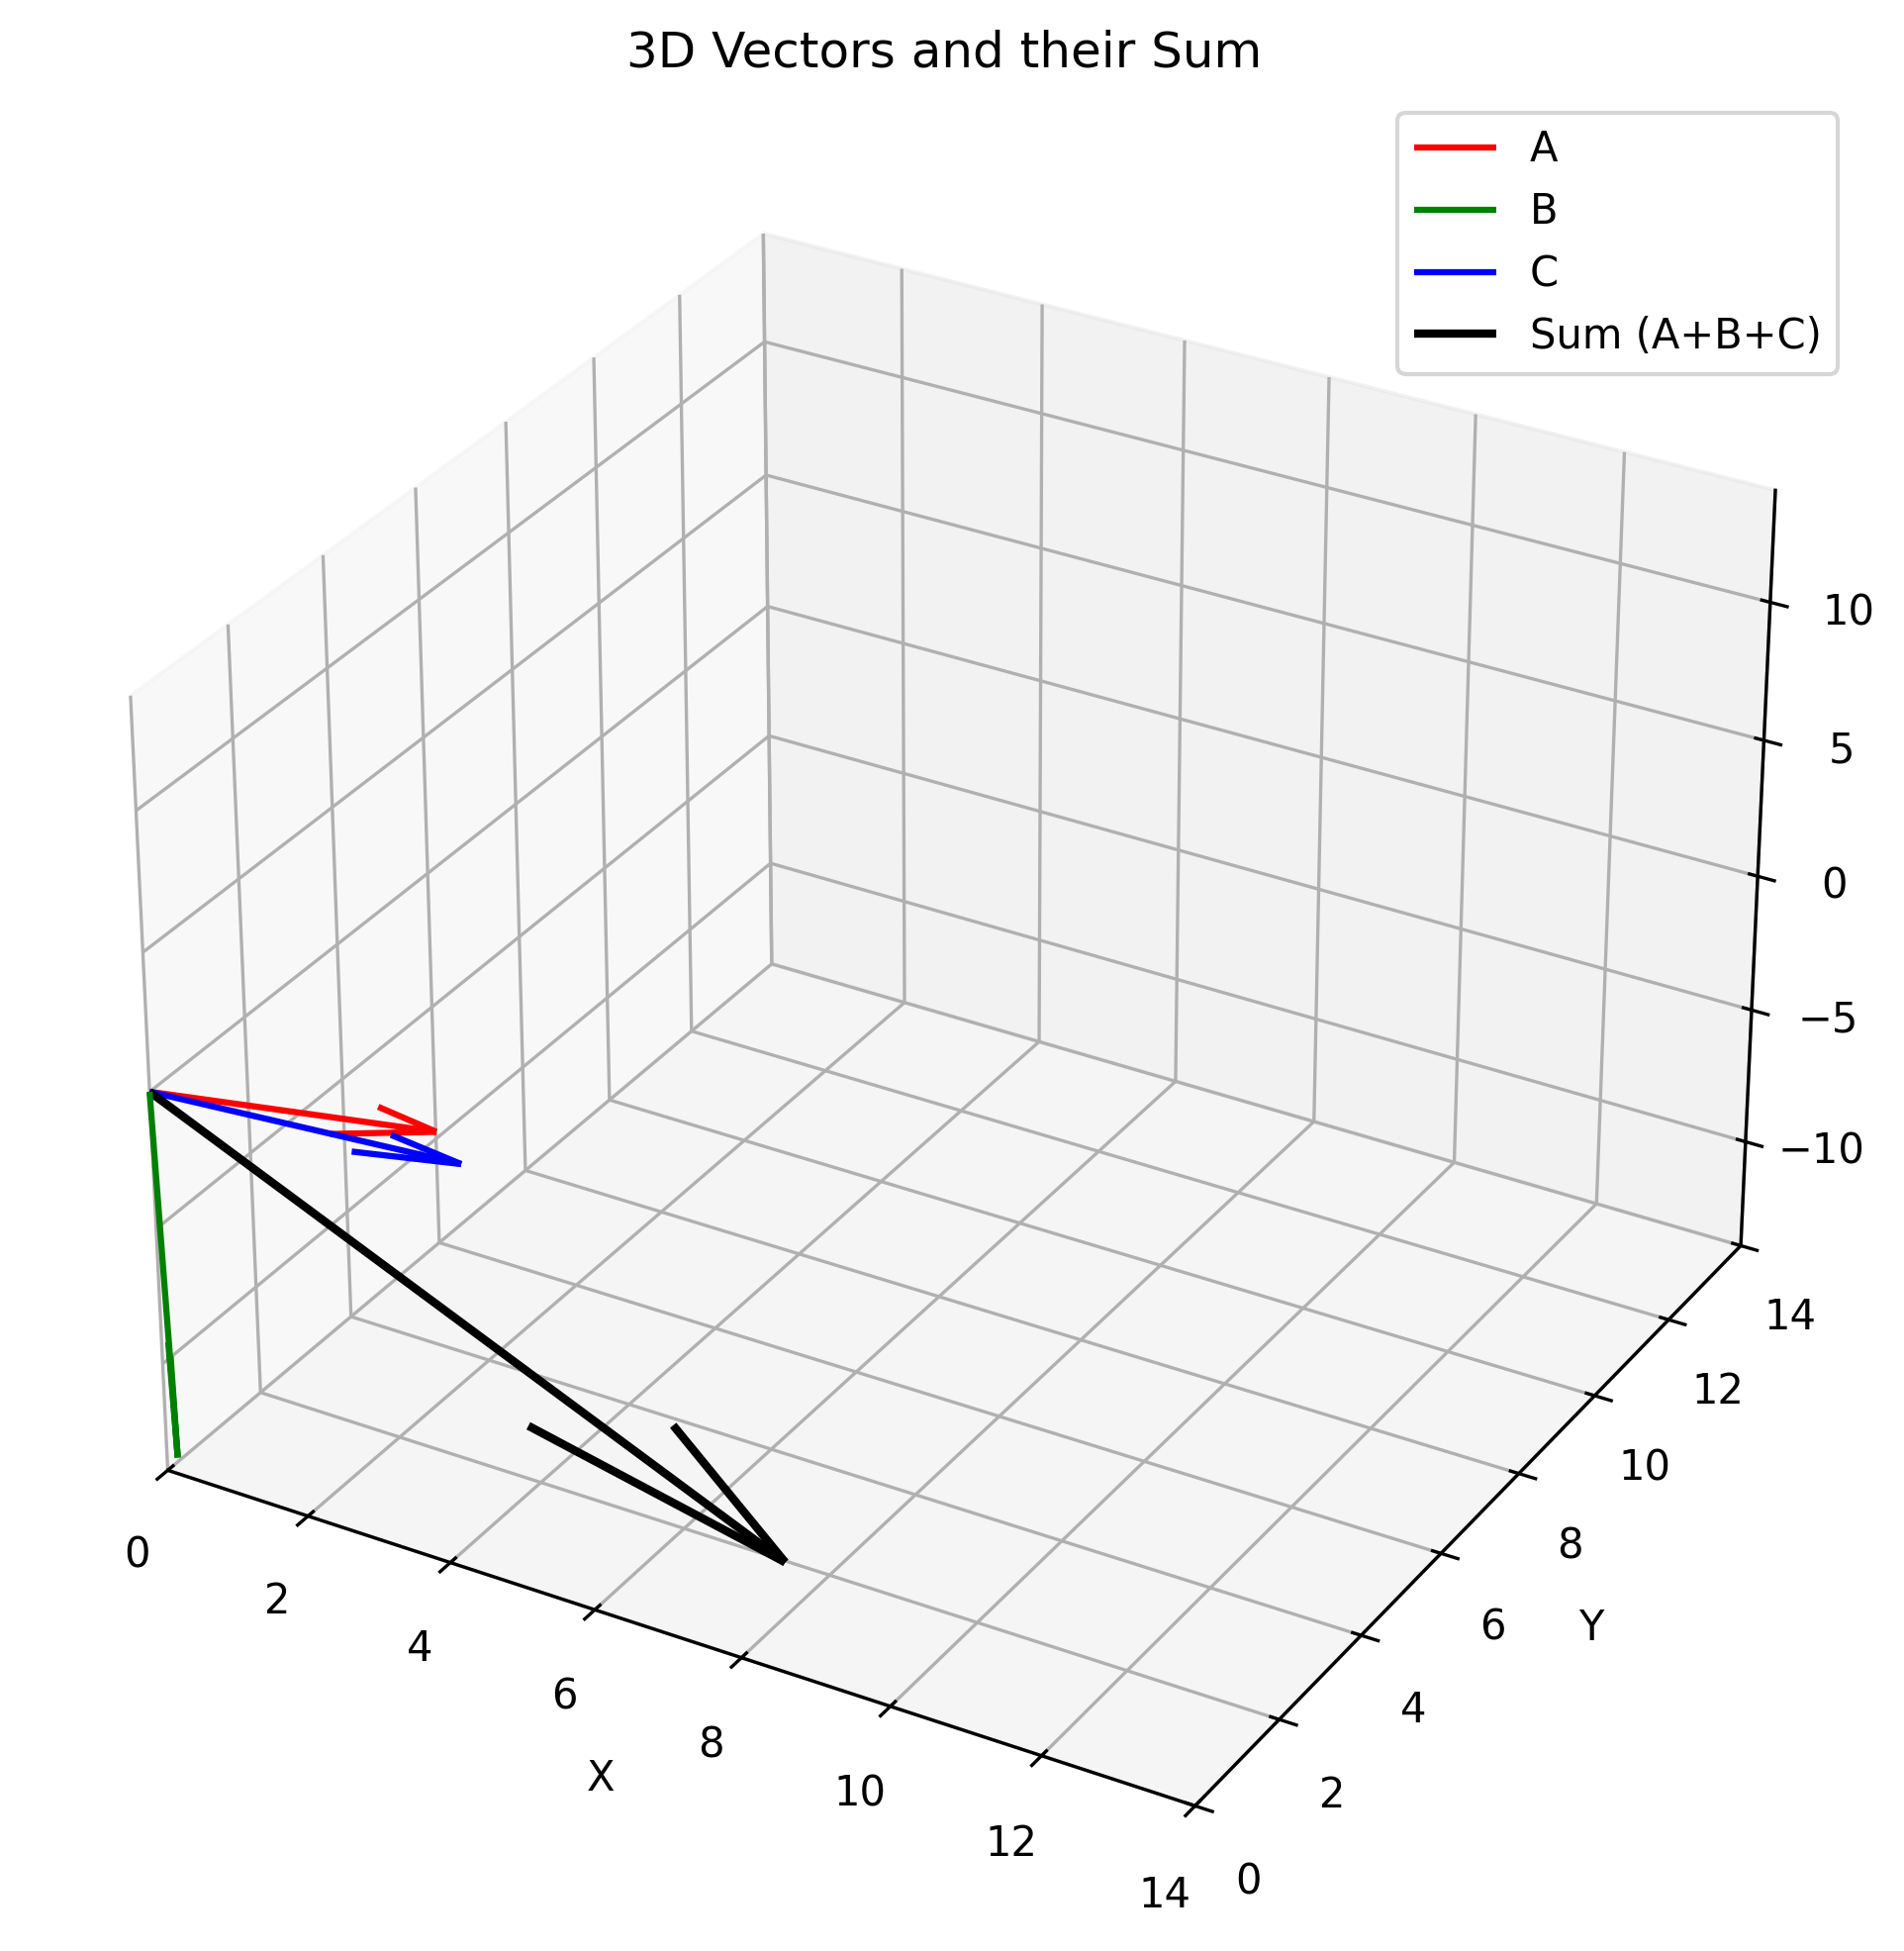
\includegraphics[width=\columnwidth, height=0.8\textheight, keepaspectratio]{figs/Figure_1.png}     
\end{frame}




\end{document}